\chapter{Introduction}
Controlling the behavior of a deformable object is difficult---
whether it is a biomechanically accurate character model or a high performance
3D printable microstructure.
Getting it right requires constant iteration, either performed manually or driven by an automated system.
These design iterations often require many expensive physical prototypes that takes months to make and test.
\begin{figure}[!htbp]
	\centering
	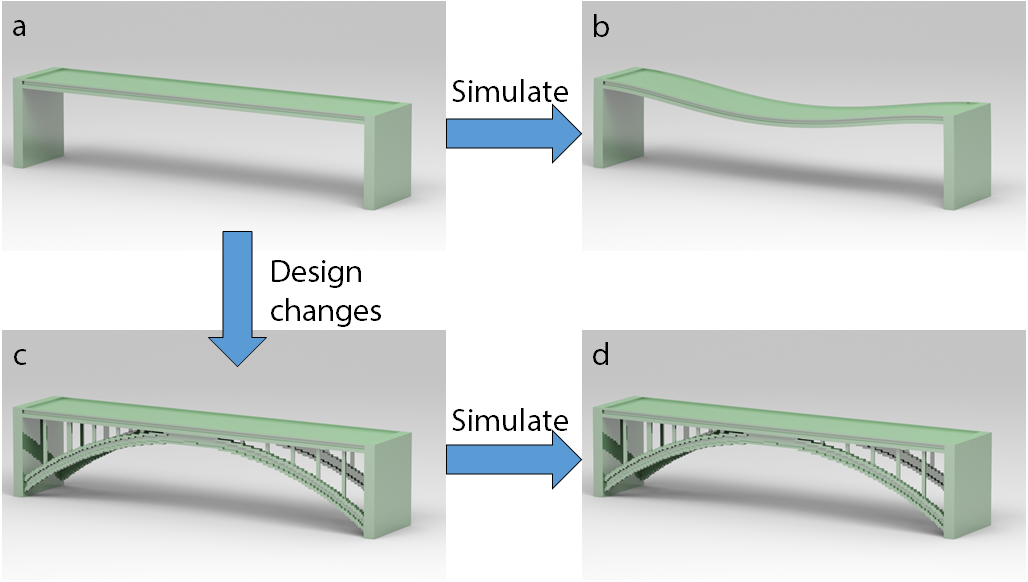
\includegraphics[width=0.8\textwidth]{images/bridgeDesign.png}
	\caption{Designing a model bridge using simulation tools.
		The bridge is made of a soft 3D-printing material. (a) Initial design.
		(b) Simulation predicts that the bridge sags significantly.
		(c) A designer adds supporting arch to the bridge.
		(d) The bridge stands without significant deformation.}
	\label{fig:bridgeDesign}
\end{figure}

Researchers and engineers use computational simulation tools to tinker with a virtual design without laboriously constructing new prototypes.
The performance of a design is predicted using computation to save time and cost of design iterations (Figure~\ref{fig:bridgeDesign}).
For such computational tools to be useful, the simulation algorithm needs to be \textit{predictive} so that simulated results agree with real-world experiments.
As a minimal requirement, the simulation should correctly predict whether a significant design modification improves or decreases the physical performance.
On top of being predictive, the simulation should be \textit{efficient} to provide interactive feedback to a designer so that she can quickly try different ideas to improve a design.

Taking a step further, a computational design algorithm can automatically tweak design parameters using a predictive simulation algorithm in the loop.
Since the simulation often needs to evaluate hundreds or thousands of design variations, the simulation still needs to be fast so that it does not take days to solve a design problem.
The gold standard technique for simulating the mechanical behavior of a deformable object is the finite element method (FEM).
While FEM is predictive to a high level of accuracy, it is notoriously slow, making it a major computational bottleneck in the iterative design process.
The slowness is because FEM is accurate only with a sufficiently high-resolution discretization.
To apply FEM to design problems, we require simulation techniques that are fast and accurate even in the face of constant tinkering.

Our goal in this thesis is to develop predictive and efficient FEM simulation tools to enable computational design optimization of deformable objects.
The key idea to achieve our goal is \textit{coarsening}.
By combining fine elements into a coarse element, the same simulation algorithm uses a much smaller number of degrees of freedom.
Since the time complexity for typical simulation algorithms grows superlinearly,
coarsening methods can quickly boost the speed of simulation algorithms.
The cost associated with coarsening is loss of accuracy.
To address this problem, we propose several different techniques to compute new material models for the coarse elements.

To test our simulation in practice, we implemented design optimization algorithms using our simulation for both static and dynamic scenarios.
For statics, we modify existing topology optimization algorithms to handle coarse elements that contain microstructures.
For dynamic problems, we use a gradient-based optimization algorithm to find locally optimal designs.

Our work draws inspiration from a diverse range of related works in computer graphics and engineering.
The next sections provide a brief review of related works on computational design, efficient FEM simulation, and topology optimization.
We then conclude this chapter by laying out thesis overview and contributions.

\section{Computational Design}
Computational design concerns itself with optimizing the shape and material assignment in an object in order to control its large scale behavior.
Advances in computational design, physical modeling and rapid prototyping 
have enabled the automated design and fabrication of objects with customized physical properties.
The range of fabrication methods and applications addressed in previous literature is very diverse spanning optical properties, inertia, aerodynamic, strength, kinematics, elasticity etc.

In the area of designing optical properties, \citet{Hasan:2010:PRO} and
\citet{Dong:2010:FSS} provided methods for printing objects with desired subsurface scattering properties. Objects have been made to reflect or bend light to create custom images \citep{papas11goal,Weyrich:2009,kiser2013}.
The inertia tensor of an object has been designed for stable standing~\citep{Prevost:2013kb}, floating~\citep{musialski-2015}
and spinning~\citep{Bacher:2014}.
The aerodynamic behavior of rigid mechanisms has been controlled to design paper airplanes~\citep{Umetani:2014}, kites~\citep{Martin:2015}, and multi-copters~\citep{Du:2016}.
Many researchers have investigated how to improve structural strength of 3D-printed objects~\citep{Stava:2012,Zhou:2013,Langlois:2016,Wu:2016,Ulu:2017}.
More complex 3D-printed mechanisms have been designed to achieve specified kinematic motions~\citep{Zhu:2012,Coros:2013:CDM,Bacher:2015,Megaro:2017}.

The most relevant line of work is the design and fabrication of deformable objects with prescribed behavior under load.
The behavior is usually controlled by altering the material
composition and shape of the designs.
\citet{Bickel:2010:DAF} used a measurement based material model to design 
layered soft structures with prescribed non-linear static deformation behavior.
\citet{Chen:2014:ANM} optimized the rest shape of a deformable object such that 
it deforms the right way under gravity.
Other researchers have used material composition and geometry to control 
articulated characters~\citep{Bickel:2012,Skouras13Computational}.
Like these works, one of our goals is to efficiently design compliant objects 
with desired deformation behavior.
These works assume a small set of available 
base materials such a stiff and a soft material.
To expand the range of material building blocks, the base materials are 
organized into larger structures known as microstructures.
These microstructures are then used in design optimization loops to 
compose objects with specified compliant 
properties~\citep{Schumacher:2015,Panetta:2015,Zhu:2017:TTO}.

\section{Efficient FEM Simulation}
As mentioned, design and fabrication of deformable objects is common in
engineering and graphics~\citep{bendsoe2004topology,Kou2012,McAdams2011}.
Efficient FEM simulation plays an important role in automating the design process.
We can broadly partition the space of approaches for
optimizing FEM simulation into two categories. We term the first
category numerical approaches. These methods use fast matrix inversion
techniques and other insights about the algebra of the FEM to increase its performance.
Simulators based on the multigrid method~\citep{Peraire1992,Zhu2010,McAdams2011}
and Krylov subspace techniques~\citep{Patterson2012} have yielded impressive performance increases.
Other hierarchical numerical approaches, as well as highly parallel techniques, have
also been applied to improve the time required to perform complex
simulations~\citep{Farhat1991,Mandel1993}.
Finally, \citet{Bouaziz:2014} have proposed specially designed energy functions and an
alternating time-integrator for efficient simulation of dynamics.

The second set of methods are reduction approaches.
These algorithms attempt to intelligently decouple or remove degrees of
freedom (DOFs) from the simulated system.
The reduction leads to smaller systems, resulting in a massive increase in performance, with some decrease in accuracy.
Our algorithm falls into this category.
Note, however, that numerical and reduction approaches need not be mutually exclusive.
For example, since our algorithm uses the same type of spatial discretization as the underlying FEM,
faster numerical algorithms such as multigrid will improve the efficiency of our algorithm.
Algorithms based on reduction approaches mitigate the inevitable increase in error using
one or more of three approaches: adaptive remeshing, higher-order
shape functions, or adaption of the constitutive model.

Adaptive remeshing alters the resolution of the simulation discretization
in response to various metrics (stress, strain, etc.). Such methods
seek to maintain an optimal number of elements and thus achieve
reasonable performance. Adaptive remeshing has proven useful
for simulating thin sheets such as cloth~\citep{Narain2012}, paper~\citep{Narain2013}, as well as elastoplastic solids~\citep{Wicke:2010} and solid-fluid mixtures~\citep{Clausen2013}.
More general basis refinement approaches have also been suggested~\citep{Debunne2001,Grinspun2002}.
While these methods do improve
the performance of simulation algorithms, they have some drawbacks.
First, they often require complicated geometric operations
which can be time consuming to implement.
Second, they introduce elements of varying size into the FEM discretization.
This can lead to poor numerical conditioning if not done carefully.
Finally, in order to maintain accuracy, it may still be necessary to introduce many
fine elements, leading to slow performance.

Alternatively, one can turn to P-adaptivity for help.
P-adaptivity refers to introducing higher-order basis functions 
to increase accuracy during simulation~\citep{Szabo2004}.
Unfortunately, these methods suffer from requiring complicated mesh generation schemes and are not
well-suited for iterative design problems.
An alternative approach to remeshing is to use higher order shape
functions to more accurately represent the object's motion
using a small set of DOFs. Modal simulation techniques fall into
this category~\citep{Shabana1991,Krysl2001,Barbic:subspace:2005}.
Substructuring~\citep{Barbic2011} decomposes an input
geometry into a collection of basis parts, performing modal reduction on each one.
These basis parts can be reused to construct new global structures.
Other approaches involve computing physically meaningful shape functions as an
offline preprocessing step.
For instance, \cite{Nesme2009} compute shape functions based on
the static configuration of a high resolution element mesh induced
via a small deformation of each vertex.
\cite{Faure2011} use skinning transformations as shape functions to simulate complex
objects using a small number of frames.
\cite{Gilles2011} show how to compute material-aware shape functions for these framebased
models, taking into account the linearized object compliance.
Both \cite{Nesme2009} and \cite{Faure2011} accurately capture
material behavior in the linear regime.
However, because their shape functions cannot change with the deformed state of the material,
they do not accurately capture the full, non-linear behavior of an elastic object.
Our non-linear coarse material models rectify this problem.
Computing material-aware shape functions improves both the speed
and accuracy of the simulation. However, these methods require a
precomputation step that assumes a fixed material distribution and geometry.
If the material distribution changes, these shape functions
must be recomputed. This step becomes a bottleneck in applications
that require constantly changing material parameters.

The final coarsening technique involves reducing the degrees of freedom
of a mesh while simultaneously augmenting the constitutive
model at each element, rather than the shape functions.
Numerical coarsening is an extension of analytical homogenization, which seeks
to compute optimal,
averaged material for heterogeneous structures~\citep{Guedes1990,farmer2002}.
Numerical coarsening, for instance, has been applied to linearly
(in terms of material displacement)
elastic tetrahedral finite elements~\citep{Kharevych2009}.
These methods require an expensive precomputation step (a series
of static solves) that must be repeated when the material content or
the geometry of an object changes.
This step holds these methods back from being suitable for iterative design problems.
\section{Topology Optimization}
Topology optimization is a class of methods for optimizing material distributions
within a design layout while satisfying given constraints~\citep{bendsoe2004topology}.
These methods typically work with linear elastic materials since it is easier to take the derivative of the objective function in this case.
Topology optimization was originally developed for structural design problems~\citep{bendsoe:1989:optimal} where the deformation is small enough to be modeled by linear elasticity.
It has been extended to a variety of problems including compliant mechanism design~\citep{Sigmund97Compliant},
mass transfer~\citep{challis:2009:level},
metamaterial design~\citep{Sigmund2000,cadman:2013:design},
multifunctional structure design~\citep{yan:2015:two},
and coupled structure-appearance optimization~\citep{Martinez:2015:SAO}.
Many algorithms have been proposed to numerically solve the optimization problem itself.
We refer to the book by~\citet{sigmund:2013:topology} for a complete review.

In the very popular SIMP (Solid Isotropic Materials with Penalization) method,
the presence of material in a given cell is controlled by locally varying its density.
A binary design is eventually achieved by penalizing intermediate values for these densities.
In practice, this method works well for two-material
designs (e.g., a material and a void), but generalizing this method
to robustly handle higher dimensional material spaces remains challenging.
Another class of methods rely on homogenization.
They replace the material in each voxel of the object by a mixture of the base materials that is known to be locally optimal for the
original problem~\citep{Allaire2012}.
While very powerful, these methods are specialized for the minimum compliance problem, for
which the link between stiffness and optimal density can be analytically formulated.
In a sense, our work can been seen as a generalization of this type of approaches to handle arbitrary materials in broader contexts.

Standard topology optimization methods suffer from a major drawback.
The parametrization of the problem at the voxel level makes them extremely expensive and impedes their use on high resolutions models such as the ones generated by modern 3D printing hardware.
To reduce the number of degrees of freedom for simulation and optimization, \citet{rodrigues:2002:h} proposed an interesting formulation where microstructure designs 
and macroscopic layouts of the underlying microstructures are hierarchically coupled and treated simultaneously.
This initial work has been extended in multiple ways~\citep{coelho:2008:h,nakshatrala:2013:non,yan:2014:concurrent,xia:2014:reduced}.
However, these methods still need to handle variables defined at
the microstructure level and therefore they remain relatively costly.
The closest to our work is probably the method proposed by~\citet{xia:2015:multiscale},
which also relies on a database to speed up computations.
However, their work specifically targets minimum compliance problem in the structural design which allows them to approximate the macroscale behaviour of the microstructures with a
particular strain-based interpolating function.
\section{Thesis Overview}\label{ch1:desc}
Chapter~\ref{ch2:ddfem} introduces FEM for simulating elastic materials.
Building on existing material models, we propose data-driven finite elements or DDFEM,
the first simulation method optimized for geometric and material design problems under static scenarios.
We improve simulation efficiency by coarsening, where we replace blocks of fine elements with coarse elements.
We then provide example energy functions for modeling coarse blocks made of heterogeneous Neo-Hookean materials.
To quickly find coarse material models for different designs, 
we use a database to store combinations of fine blocks and their corresponding elastic potential energy functions.

Chapter~\ref{ch3:topopt} proposes to represent the space of material properties as a level set.
The level set representation can be used to sample the space of heterogeneous materials more efficiently.
For this study, we restrict the coarse material blocks to be composed of linear base materials.
The coarse material blocks are assumed to be tiled with the same or similar blocks in a periodic pattern.
With these assumptions, we can sample the space of coarse blocks at a much higher resolution.
These high resolution material blocks are called microstructures.
We computed the material property space of cubic-symmetric microstructures and discovered families of microstructures that achieves extremal elastic properties.
In addition, the level set representation is incorporated into topology optimization algorithms to automatically design objects made of microstructures instead of homogeneous material blocks.
This two-scale topology optimization method allows us to design high-resolution objects such as a functional gripping mechanism and a bridge model with maximum stiffness.

Chapter~\ref{ch4:desdyn} investigates the possibility of designing real-world high-speed dynamic mechanism using coarsened simulations.
We propose dynamics-aware coarsening (DAC) to model the dynamic elastic behavior using coarse elements.
For impact modeling, we propose boundary-balancing impact (BBI) to model the inelastic impact of elastic objects.
With these methods, we optimize and fabricate jumping mechanisms that are challenging to design by hand.
\section{Contributions}
\begin{itemize}
	\item DDFEM is the first algorithm for fast runtime coarsening of nonlinear elastic models that can handle changing geometry and material assignment.
	DDFEM first precompute the material properties of coarse elements composed of fine elements with different materials.
	This is done by computing the deformations of coarse elements under likely forces.
	A compact material model is developed to represent the coarse element behavior in a compact form.
	\item Two-scale topology optimization modifies the existing topology optimization methods to incorporate gamut constraints.
	Instead of optimizing material mixture ratio at each cell, our approach optimizes the material properties at each cell within material property gamut.
	This ensures that the final result is realizable by mapping each cell to a microstructure with the optimized material properties.
	\item Efficient microstructure sampling methods lead to the computational discovery of microstructure families with extremal elastic properties.
	Starting with voxel representation of microstructures,
	our method automatically cluster similar structures into families and extract parametric templates from the families.
	The templates are controlled by a small number of parameters to allow more efficient sampling and tweaking.
	They also reveal the underlying structural similarity that are crucial achieving the extremal physical properties.	
	\item Dynamics-aware coarsening (DAC) computes coarse material properties geared towards dynamic scenarios.
	The material parameters are computed such that the primary modal frequency
	of a coarse mesh matches the frequency of a high resolution mesh or a physical model.
	This allows us to simulate dynamic trajectories of non-linear elastic objects at much faster rates while still matching the macroscopic behavior.
	\item Boundary-balancing impact (BBI) improves state of the art impact models to more accurately model real-world inelastic impact.
	The combination of DAC and BBI allows us to simulate and predict the behavior of elastic jumping mechanisms.
	The simulation is predictive and efficient enough to be used in design optimization loops to improve the designs of real-world jumping mechanisms.
\end{itemize}